\documentclass{minimal}
\usepackage{tikz}

\begin{document}
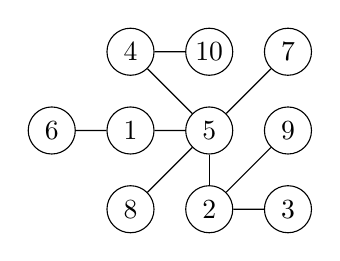
\begin{tikzpicture}
\tikzstyle{vertex}=[circle, draw, minimum size=17pt, inner sep=0pt]
\node[vertex] (1) at (0,1) {1};
\node[vertex] (2) at (1,0) {2};
\node[vertex] (3) at (2,0) {3};
\node[vertex] (4) at (0,2) {4};
\node[vertex] (5) at (1,1) {5};
\node[vertex] (6) at (-1,1) {6};
\node[vertex] (7) at (2,2) {7};
\node[vertex] (8) at (0,0) {8};
\node[vertex] (9) at (2,1) {9};
\node[vertex] (10) at (1,2) {10};

\draw (6)--(1)--(5)--(8);
\draw (10)--(4)--(5)--(7);
\draw (9)--(2)--(3);
\draw (2)--(5);

  \end{tikzpicture}

\end{document}
